\documentclass[UTF8,noindent]{ctexart}
\usepackage[a4paper,left=2.0cm,right=2.0cm,top=2.0cm,bottom=2.0cm]{geometry}
\usepackage{graphicx}
\usepackage{amsmath}
\usepackage{amssymb}
\usepackage{xeCJK}
\usepackage{listings}
\usepackage{float}
\CTEXsetup[format={\Large\bfseries}]{section}

\title{$Project2\quad Non-Preemptive Kernel$ 设计文档}

\author{冯吕$\quad 2015K8009929049$}
\date{\today}
\begin{document}
\maketitle
\zihao{5}
\CJKfamily{zhsong}


\section*{一、Content Switching 设计流程}
在本次任务中,需要实现一个非抢占式的调度器,以及多$task$的启动和\emph{content 
switch}。在设计过程中,首先,需要确定$PCB$保存的信息,即进程控制块信息。根据简单分析可知,$PCB$需要
保存的信息如下:
\begin{itemize}
	\item $sp$:栈指针,栈指针指向进程当前栈的位置,因此在上下文切换的时候需要进行保存。
	\item $ra$:$ra$保存着返回地址,因此需要保存。
	\item $s_0 \sim s_7$:这$8$个寄存器会保存寄存器变量,因此需要保存。
	\item 进程状态。
\end{itemize}

上下文切换时,只需要保存上面这些信息,其他寄存器的值不再需要保存,比如$a_0 \sim 
a_3$,尽管它们保存着函数参数,但是如果进程切换回来之后还需要使用这些参数,那么它会在进程切换前先将这些参数压栈,
因此不需要保存。

启动进程时,首先需要初始化进程的调度队列,初始化$PCB$,初始化$PCB$时,将$s_0\sim 
s_7$这八个寄存器的值均初始化为$0$,$ra$的值设置为进程/线程的地址,$sp$设置为进程的栈起始地址。初始化完成之后,便调用
$scheduler\_entry()$函数加载准备队列中的第一个进程运行。

当进程运行过程中遇到$yield()$函数,或进程运行中遇到$do\_yiled()$函数,则进行进程切换。线程切换时,$
do\_yiled()$函数首先调用$save\_pcb()$函数保存当前进程的$PCB$信息,并$push$到准备队列中,然后调用
$scheduler\_entry()$函数启动新的进程。$scheduler\_entry()$调用$scheduler()$函数$pop()$一个
进程到$current\_running$中,然后将$PCB$中保存的寄存器值加载到寄存器中,之后跳到$ra$所在地址继续运行。
若是进程遇到$yield()$函数,则通过系统调用来调用$do\_yield()$来切换进程。

下面是简单的函数调用关系:
\begin{itemize}
	\item $bootblock\text{读盘}\Rightarrow \_stat()$\\
	$\_stat()$函数完成$PCB$的初始化和准备队列的初始化,之后调用$scheduler\_entry()$启动进程(线程$1$);
	
	\item $scheduler\_entrry()\Rightarrow scheduler()\Rightarrow$启动第一个进程
	\item 线程切换:$do\_yield()\Rightarrow save\_PCB() \&\& queue\_push 
	\&\&scheduler\_entry()$
	\item 进程切换:$yield()\Rightarrow \text{系统调用}\Rightarrow do\_yield()$
\end{itemize}

上下文切换时,需要保存$PCB$,主要是将寄存器的值保存到$PCB$中,对于$s_0\sim 
s_8$这八个寄存器,直接保存即可,而对于$sp$和$ra$,则需要特殊对待,上下文切换时需要保存的是调用$do\_yiled()$
函数时候的$sp$和$ra$的值,但是,当$do\_yiled()$函数调用$save\_pcb()$函数的时候将需要保存的$ra$压栈了,$ra$变成了$save\_pcb()$的返回地址,
并且栈的地址也减小了$24$,所以,在$save\_pcb()$中,需要将$sp+24$保存到$PCB$中,以及压在栈中的$ra$保存到$PCB$中。\\

$bootblock$的传参: 

在实验一中,我是直接修改指令实现传参,但是,这样实际上我需要事先知道指令地址,因此并不是一个好的方法。在实验二中,我改为将参数写到$bootblock$这一扇区最后为$0$的其中一个位置,然后在
$bootblock$中通过$lw$指令将参数加载到寄存器中。

运行截图:
\begin{figure}[H]
	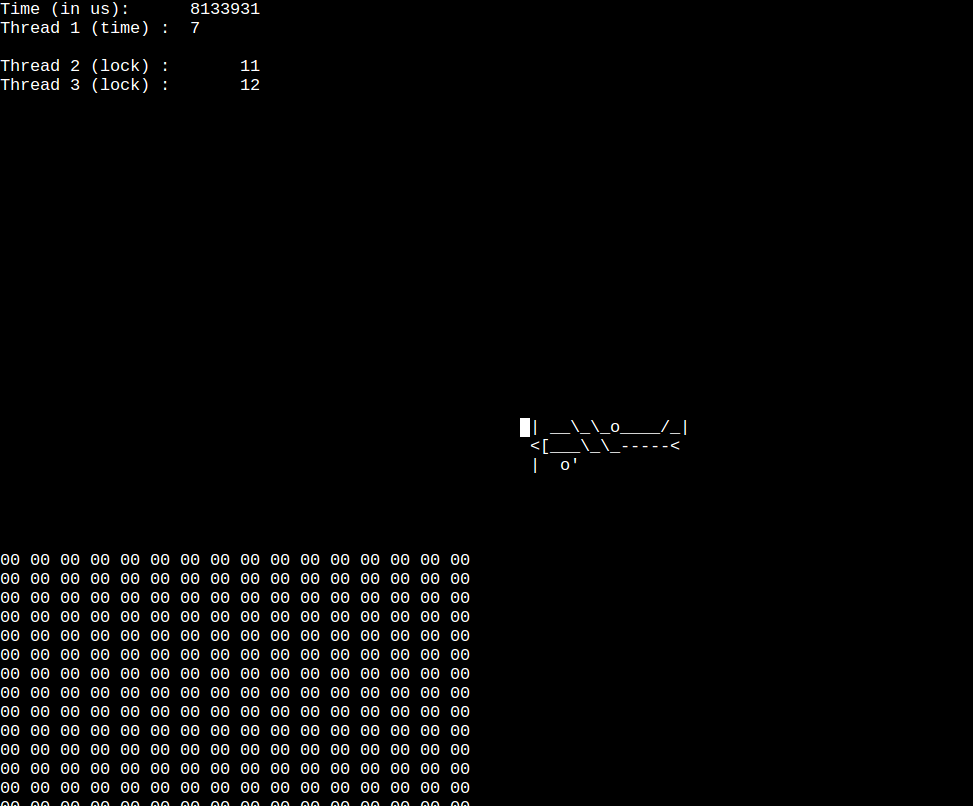
\includegraphics[scale=0.5]{fig/1.png}
\end{figure}

\section*{二、Content Switching 开销测量}
对于线程切换到线程和进程切换到进程的开销测量,可直接利用全局变量来测量,当一个进程执行$yiled()$
函数之前调用$get\_timer()$函数获取一次时间,切换到下一个进程里面再测量一个时间,两个时间的差便是
进程之间切换的时间开销。线程和线程之间的切换也是同样的测量。

对于线程和进程之间的切换,则有所不同,由于线程和进程之间不同共享变量,因此,上面的方法行不通,解决办法就是,
当从线程切换到进程之后,立刻又切换回线程,从而算出两次切换的时间和,除以二便可得到线程和进程之间上下文切换的开销
。

运行截图:
\begin{figure}[H]
	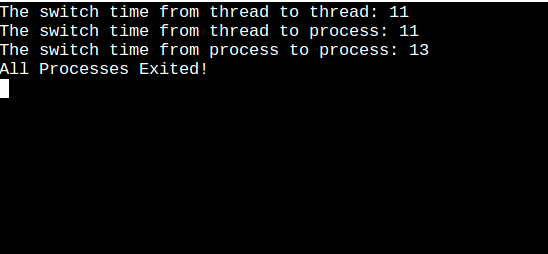
\includegraphics[scale=0.7]{fig/2.png}
\end{figure}

\section*{三、互斥锁的设计}
任务三中,需要设计一个实现进程调度的互斥锁。互斥锁的设计是为了保证共享数据操作的完整性。

自旋锁与互斥锁功能类似,都是为了解决对某项资源的互斥使用。无论是互斥锁,还是自旋锁,
在任何时刻,最多只能有一个保持者,也就说,在任何时刻最多只能有一个线程能够获得锁。
但是两者在调度机制上略有不同。对于互斥锁,如果资源已经被占用,资源申请者只能进入睡眠状态。
但是自旋锁不会引起调用者睡眠,如果自旋锁已经被别的线程占用,调用者就一直循环在那里看是否
该自旋锁的保持者已经释放了锁。

对于互斥锁,线程如果获取锁成功,那么便可以执行,如果获取锁失败,那
么就会进入$block$状态,即被压入$block$队列。被阻塞后的线程只有等到$unblock$之后获得了锁才能
够继续执行。

运行截图:
\begin{figure}[H]
	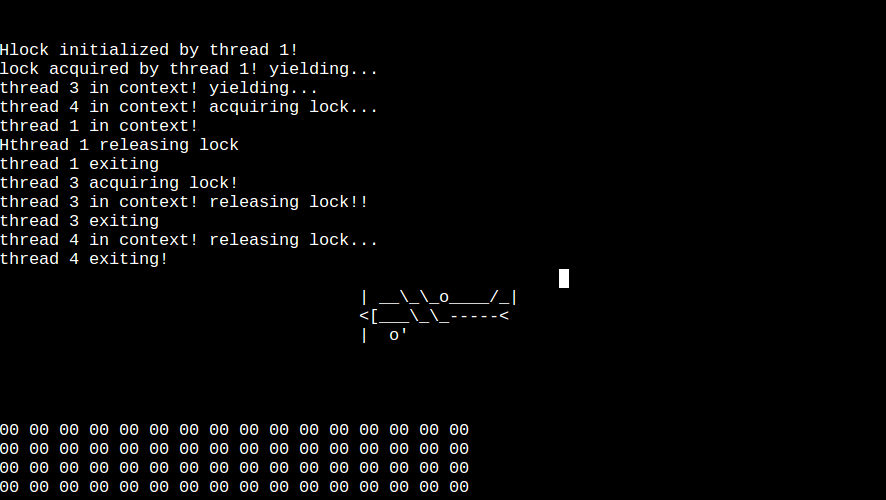
\includegraphics[scale=0.5]{fig/3.png}
\end{figure}
全部测试截图:
\begin{figure}[H]
	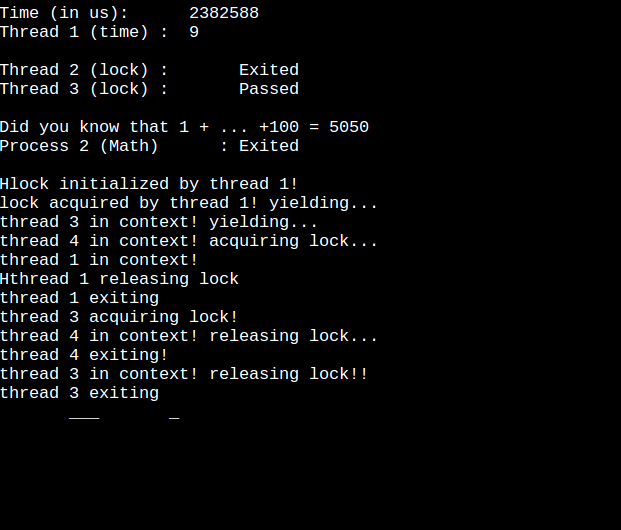
\includegraphics[scale=0.5]{fig/4.png}
\end{figure}

\section*{四、关键代码片段}

1.$scheduler\_entry()$函数:
\begin{lstlisting}[language =c]
scheduler_entry:

la t0, scheduler
jal t0

lw t1, (current_running)
lw s0, 0(t1)
lw s1, 4(t1)
lw s2, 8(t1)
lw s3, 12(t1)
lw s4, 16(t1)
lw s5, 20(t1)
lw s6, 24(t1)
lw s7, 28(t1)
lw sp, 32(t1)
lw ra, 36(t1)

jr ra;
\end{lstlisting}
该函数首先调用$scheduler()$函数弹出一个新的进程到$current\_running$,然后将相应值加载到寄存器中
,再跳到$ra$所在的位置执行,因此,初始化$PCB$时,存储$ra$的位置存的就是进程的地址。

2.$save\_pcb()$函数:
\begin{lstlisting}[language=c]
save_pcb:
la t0, current_running 
addiu sp, sp, 24
lw t1, (current_running)
sw s0, 0(t1)
sw s1, 4(t1)
sw s2, 8(t1)
sw s3, 12(t1)
sw s4, 16(t1)
sw s5, 20(t1)
sw s6, 24(t1)
sw s7, 28(t1)
sw sp, 32(t1)  # save sp
addiu sp, sp, -24
lw t2, 16(sp) # save ra
sw t2, 36(t1)
jr ra
\end{lstlisting}
该函数将寄存器的值保存到$PCB$中,需要注意的是$sp$和$ra$的值在调用函数的过程中会发生变化,
因此保存时候需要特殊处理。

3.$\_stat()$函数:
\begin{lstlisting}[language=c]
void _stat(void){

  blocked_queue = &block_queue;
  ready_queue = &task_queue;
  queue_init(ready_queue);
  queue_init(blocked_queue);

  clear_screen(0, 0, 30, 24);

  int i, j;
  ready_queue->capacity = NUM_TASKS;
  ready_queue->pcbs = ready_array;
  for (i = 0; i < NUM_TASKS; i++ ){
    for (j = 0; j < NUM_REGISTERS; j++ )
      ready_arr[i].reg[j] = 0;
    ready_arr[i].sp = STACK_MAX - i * STACK_SIZE ;
    ready_arr[i].ra = task[i]->entry_point;
    ready_arr[i].state = PROCESS_READY;
  }
  ready_queue->pcbs = ready_array;
  for ( i = 0; i < NUM_TASKS; i++ )
    queue_push(ready_queue, &ready_arr[i]);

  blocked_queue->pcbs = blocked_arr;
  blocked_queue->capacity = NUM_TASKS;

  scheduler_count = 0;
  scheduler_entry();

  ASSERT(0);
}
\end{lstlisting}
该函数是内核中最开始执行的函数,它需要完成$PCB$的初始化,然后启动第一个进程。初始化$PCB$时候,
$sp$初始化为进程栈的位置,$ra$初始化为进程的地址,其余寄存器的值初始化为$0$。

4.$do\_yiled()$函数:
\begin{lstlisting}[language =c]
void do_yield(void)
{
  save_pcb();
  current_running->state = PROCESS_READY;
  /* push the qurrently running process on ready queue */
  queue_push(ready_queue, (pcb_t *)current_running);

 // call scheduler_entry to start next task
  scheduler_entry();

// should never reach here
  ASSERT(0);
}
\end{lstlisting}
该函数首先调用$save\_pcb()$函数将当前正在运行的进程的状态保存下来,然后压入准备队列,再从准备队列中
加载下一个进程运行。

5.$lock()$函数:
\begin{lstlisting}[language=c]
void block(void)
{
  save_pcb();

  current_running->state = PROCESS_BLOCKED;
  queue_push(blocked_queue, (pcb_t *)current_running);

  scheduler_entry();
  ASSERT(0);
}
\end{lstlisting}
需要锁的线程如果获取锁失败,则被压入$block$队列,只有等到当前拥有锁的线程释放了锁,它获得了锁,
才能够重新运行。

6.$un\_block()$函数:
\begin{lstlisting}[language=c]
int unblock(void)
{
  if (blocked_tasks()){
    unblock_pcb = queue_pop(blocked_queue);
    unblock_pcb->state = PROCESS_READY;
    queue_push(ready_queue, (pcb_t *)unblock_pcb);
    return 1;
  }
  return 0;
}
\end{lstlisting}
当线程释放锁以后,需要调用该函数,如果$block$队列中有被阻塞的线程,那么把它加入准备队列,同时
返回$1$,否则返回$0$,以便确定$un\_block()$执行完以后锁的状态。
\end{document}

